The purpose is to predict the total hourly wind production available on the energy market from all of western Denmark (DK1). It is important to note that it is the wind production available on the market and not the entire production of Western Denmark. This can also be seen by the correlation between demand and wind production in Table~\ref{table:pearsonCoeficientWindProduction} which indicates that the production is moved into the market when the demand for electricity is high. Because the wind production follows demand and thereby the market there is a potential in considering  economical and statistical factors of the current market situation when predicting the wind power. It is our intention to get a close enough estimate so that it can be used as an indicator for the hourly amount of wind production in the market for the next 24 hours.
Most others have been forecasting the wind production for specific wind farms where exact weather conditions and wind mill throughput of the site is known beforehand. The assumption is that we lose accuracy without the actual throughputs of the windmills because it is directly proportional to the meteorological factors as presented in~\ref{sec:windmillPlacement}. 

The \fnurl{Pearson Correlation Coefficient}{http://en.wikipedia.org/wiki/Pearson_product-moment_correlation_coefficient} has been used to establish the linear dependency between meteorological factors, demand and wind production. Table ~\ref{table:pearsonCoeficientWindProduction} shows this correlation coefficients. The influential factors will be elaborated in this section. Demand and wind speed has the immediate best correlation to wind power. The analysis will look further into all of the parameters.

\begin{table}[H]
\centering  % used for centering table
\begin{tabular}{|c|c|} % centered columns (3 columns)
\hline
Input factor & Pearson Correlation to Wind Power \\ 
%heading
\hline                  % inserts single horizontal line
Demand & 0.61 \\ \hline % inserting body of the table
Wind Speed & 0.94 \\ \hline
Temperature & -0.09 \\ \hline
Wind Direction & 0.21 \\
\hline %inserts single line
\end{tabular}
\caption{Table showing Pearson correlation coefficient between various factors and the wind production.} % title of Table
\label{table:pearsonCoeficientWindProduction} % is used to refer this table in the text
\end{table}

\subsection{Meteorological factors}
It is not surprising that weather conditions directly impact the wind power generation. The typical input parameters for wind power prediction are wind speed, air density, temperature and pressure \cite{WindPowerGenerationUsingANN} with the most influential factor being wind speed because it is directly converted to power in the wind turbine. The following will describe the parameters relationship to wind production and how it is used in the modelled ANN.

\subsubsection{Wind Speed}
\label{sec:windPowerWindSpeed}
Wind speed is directly proportional to wind production as described in Section~\ref{sec:windmillPlacement}. To illustrate this relationship 300 hours that are considered representative is showed in Figure~\ref{fig:windVsProd}.  The graph shows the expected relationship in the way wind power follows the trend of the wind speed (this must be differentiated from the predictions graphs so have extra attention on the two axes with different values here). Finally a plot diagram all of 2012 with the correlation coefficient is shown in Figure~\ref{fig:windSpeedWindProductionPlot} which makes no room for doubting the influence of wind speed on wind power. A final remark is how wind speed covers a wide range of wind power productions over the year --- as an example consider wind speed 15 and how it covers wind power in the interval of approximately 700 to 1900. The ANN generalization will move the function towards the majority of the interval but when facing the less represented values they will be hard to predict. It can become an issue that must be looked into during experiments.  

\begin{figure}[H]
\centering
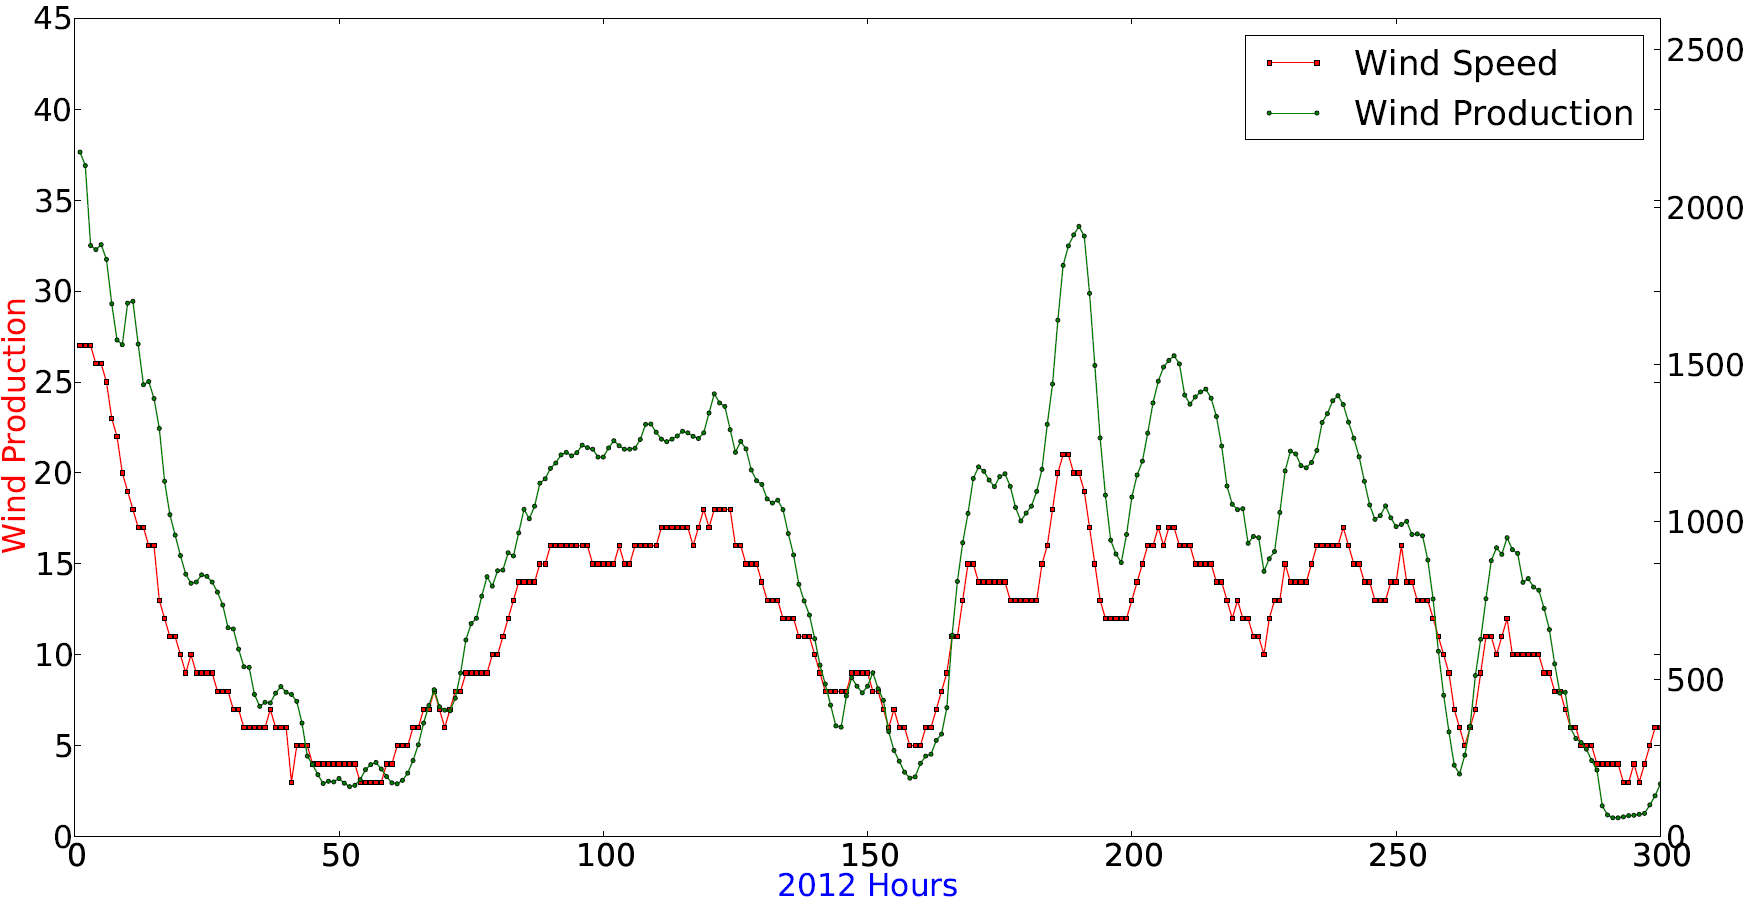
\includegraphics[width=0.99\linewidth]{billeder/windSpeedWindProductionPlot.png}
\caption{Wind speed and wind production in diagram}
\label{fig:windSpeedWindProductionPlot}
\end{figure}

\begin{figure}[H]
\centering
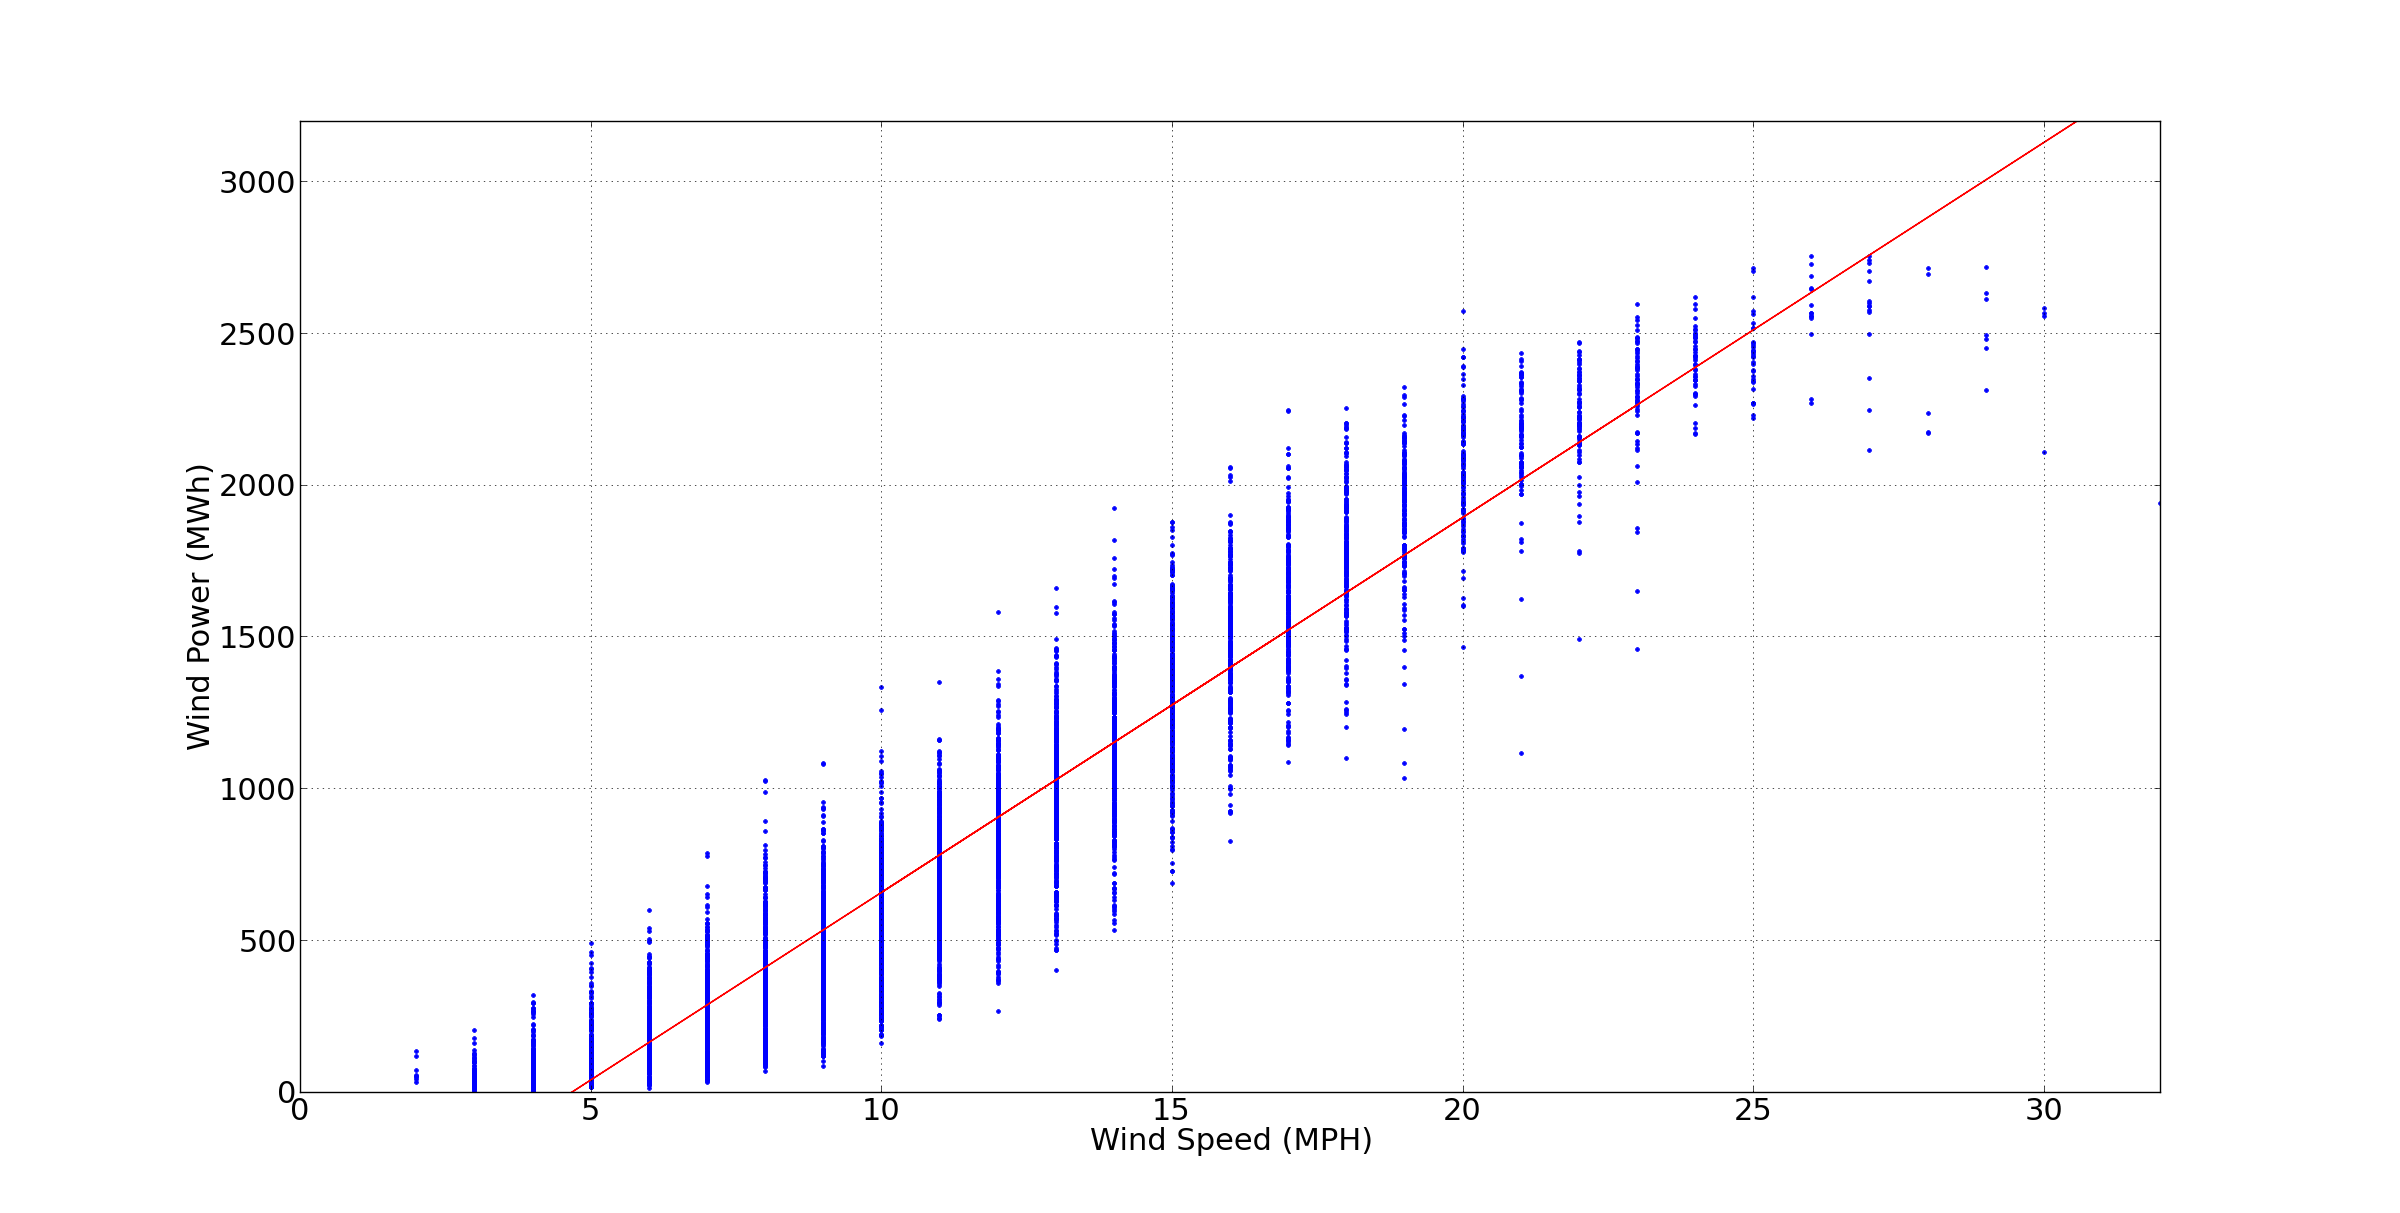
\includegraphics[width=0.95\linewidth]{billeder/WindSpeedVsProduction.png}
\caption{Wind speed vs. wind production from 2012}
\label{fig:windVsProd}
\end{figure}

\subsubsection{Air Density}
\label{sec:airDensity}
It is described in Section~\ref{sec:windmillPlacement} that wind energy is proportional to air density where a higher density means more power for a specific wind speed. This is expressed in the formula $Power from Wind=\frac{1}{(2)}*\rho*A*V^3$ where $\rho$ = air density, A = area of wind turbine and V = wind speed. The wind speed is obviously more influential and we must find out the influence of air density on all different wind speeds in order to identify its significance, e.g. consider the hypothetical examples of wind power calculations below:
\\[0.5cm]
\noindent Example 1:

\begin{center}
$wind power = \frac{1}{(2)}*0.9*1*10^3 = 450$
\end{center}

\noindent where where V = 10, A = 1 and $\rho$ =  0,9.
\\[0.5cm]
\noindent Example 2: 

\begin{center}
$wind power = \frac{1}{(2)}*0.1*1*22^3 = 532$
\end{center}

\noindent where V = 22, A = 1 and $\rho$ =  0,1.
\\[0.5cm]
\noindent It illustrates why air density cannot be compared directly to wind power. Even though air density is much higher in the first example it still has a lower wind power than the second example due to the wind speed.

Air density depends directly on temperature and pressure which can be described by $Air Density=\frac{P*M}{(R*T)}$ where R is a gas constant, M is the mass of dry air, P is pressure and T is temperature. The monthly pressure in Denmark has low variation compared to the temperature as shown in Figure~\ref{fig:pressureTemperatureVariance}. For this reason, the temperature will have the most influence on the air density in Denmark and it might even be enough to leave out pressure and only include temperature. The formula express that when temperature decreases the air density will increase, e.g. the wind power production for a specific wind speed will be higher in times of low temperature. The air density has been calculated for every hour in the training set and the correlation has been established for each wind speed in Table~\ref{table:pearsonCoeficientAirDensity}. The wind power production increases with the air density for each wind speed as described by the formula but how much varies from wind to wind speed --- wind speed 24 and the various air densities have no influence on wind power but in average the influence of air density is seen in a correlation of 0,28.

\begin{figure}[H]
\centering
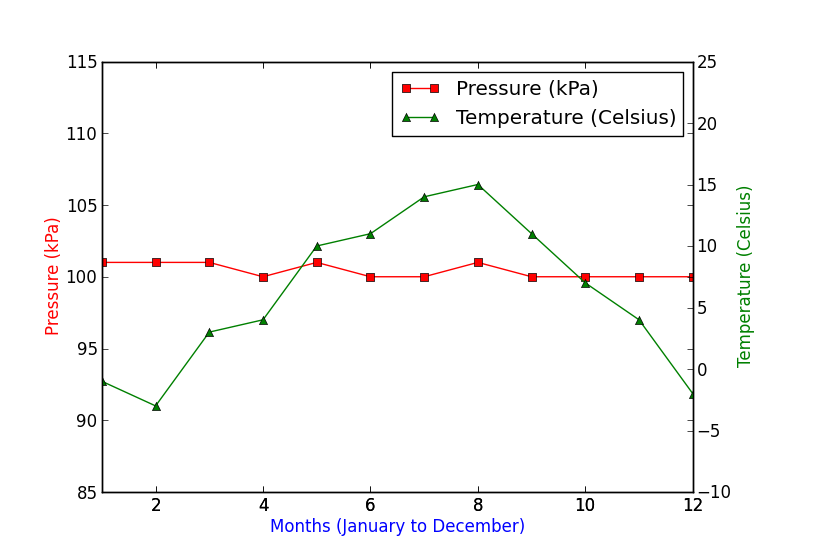
\includegraphics[width=0.95\linewidth]{billeder/pressureTemperatureVariance.png}
\caption{Temperature and Pressure variance for 2012}
\label{fig:pressureTemperatureVariance}
\end{figure}

\footnotesize
\begin{table}[H]
\centering  % used for centering table
\begin{tabular}{|c|c|} % centered columns (3 columns)
\hline
Wind Speed (mph) & Co-relation between air density and wind power \\ % inserts table 
%heading
\hline                  % inserts single horizontal line
2 & 0,29\\ \hline
3 & 0,38 \\ \hline
4 & 0,28 \\ \hline
5 & 0,18 \\ \hline
6 & 0,27 \\ \hline
7 & 0,26 \\ \hline
8 & 0,29 \\ \hline
9 & 0,31 \\ \hline
10 & 0,28  \\ \hline
11 & 0,18 \\ \hline
12 & 0,19 \\ \hline
13 & 0,19 \\ \hline
14 & 0,19 \\ \hline
15 & 0,12 \\ \hline
16 & 0,10 \\ \hline
17 & 0,22 \\ \hline
18 & 0,11 \\ \hline
19 & 0,28 \\ \hline
20 & 0,11 \\ \hline
21 & 0,18 \\ \hline
22 & 0,18 \\ \hline
23 & 0,26 \\ \hline
24 & 0,01 \\ \hline
25 & 0,12 \\ \hline
26 & 0,20 \\ \hline
27 & 0,72 \\ \hline
28 & 0,87 \\ \hline
29 & 0,61 \\ \hline
30 & 0,76 \\ \hline  
Average: & 0,28 \\ % [1ex] adds vertical space      
\hline %inserts single line
\end{tabular}
\caption{Table showing Pearson correlation coefficient between the various wind speeds in the dataset and the air density.} % title of Table
\label{table:pearsonCoeficientAirDensity} % is used to refer this table in the text
\end{table}
\normalsize

\subsubsection{Wind Direction}
Figure~\ref{fig:windDirVsProd} shows that the wind direction in general has a slight impact on the wind production (even though it is hard to see from the plot) which can also be seen in the correlation constant 0,21 from Table~\ref{table:pearsonCoeficientWindDirection}. The wind direction is expected to have a small influence based on Section~\ref{sec:windmillPlacement} where it is described how change in wind direction affect placement of windmills. The wind speed could be more powerful when coming from a specific direction which differs according to the physical location. It needs to be validated in experiments if the wind direction makes sense for western Denmark.
 
\begin{table}[H]
\centering  % used for centering table
\begin{tabular}{|c|c|} % centered columns (3 columns)
\hline
Input factor & Pearson Correlation Coefficient \\ % inserts table 
%heading
\hline                  % inserts single horizontal line
Wind Production & 0.21 \\ \hline % inserting body of the table
Wind Speed & 0.20 \\ \hline % [1ex] adds vertical space
\hline %inserts single line
\end{tabular}
\caption{Table showing Pearson correlation coefficient between various factors and the wind direction.} % title of Table
\label{table:pearsonCoeficientWindDirection} % is used to refer this table in the text
\end{table}

\begin{figure}[H]
\centering
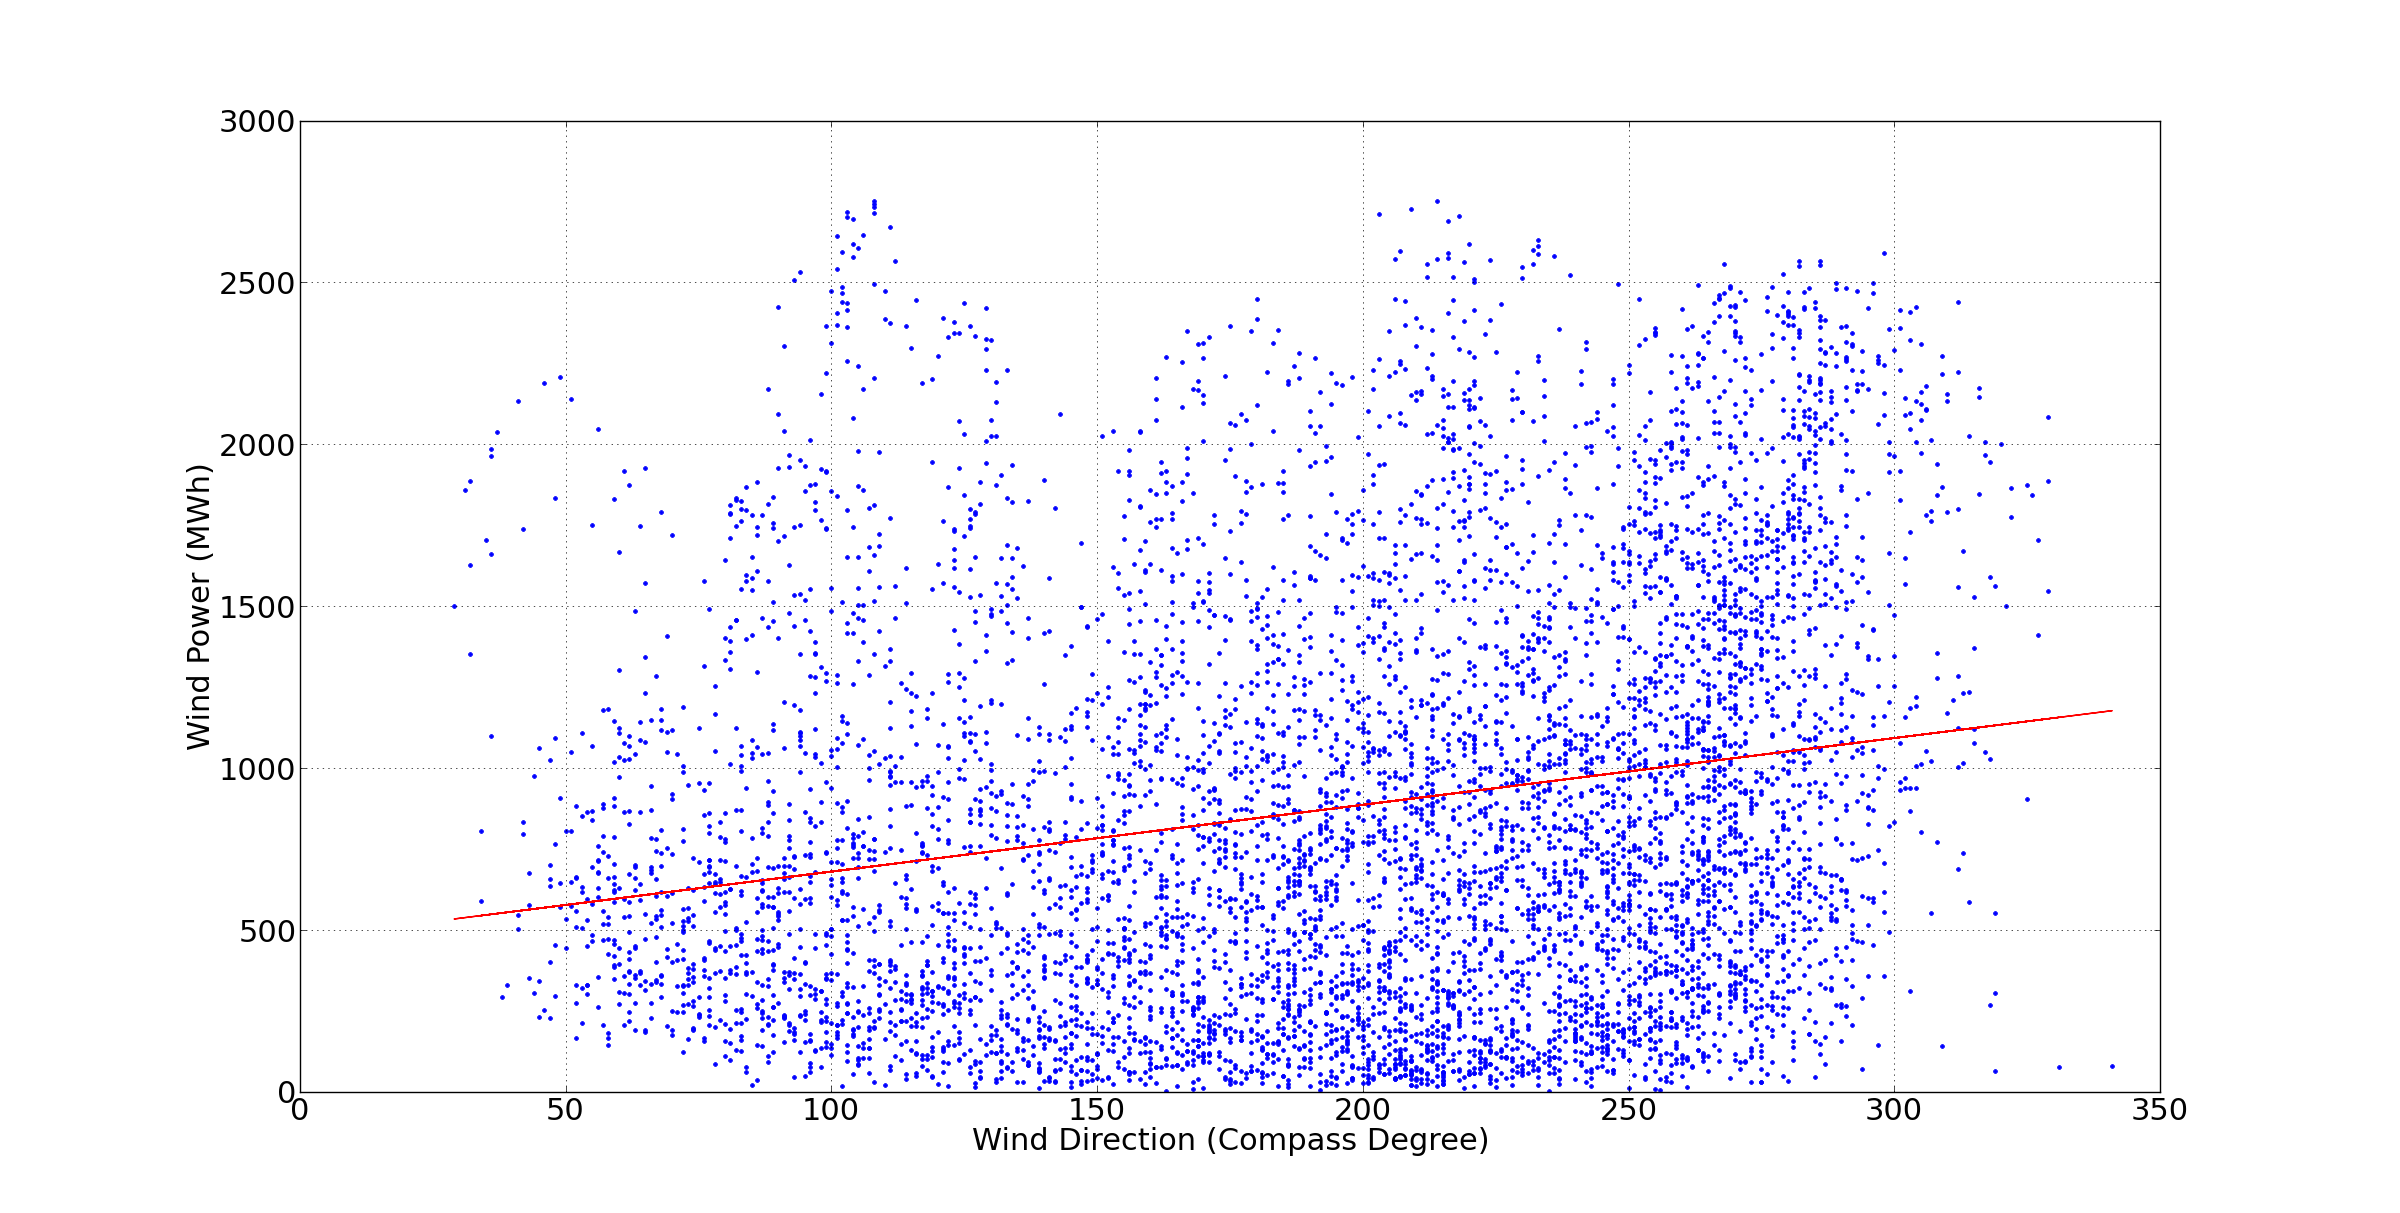
\includegraphics[width=0.95\linewidth]{billeder/productionVsWindDirection.png}
\caption{Wind Direction vs. wind production in 2012}
\label{fig:windDirVsProd}
\end{figure}

\subsection{Demand}
\label{sec:demandWindProduction}
According to the correlation constant of 0.61 from Table~\ref{table:pearsonCoeficientWindProduction} it is expected that the available wind power on the electricity market will be low at times with low demand, e.g if no energy is needed the wind power can't be sold.  The relationship is shown in Figure~\ref{fig:demandVsWindProduction} where wind power illustrates its relationship with demand in the plot diagram. It tells us that the wind production is connected to the market and cannot be deduced only from meteorological factors.

\begin{figure}[H]
\centering
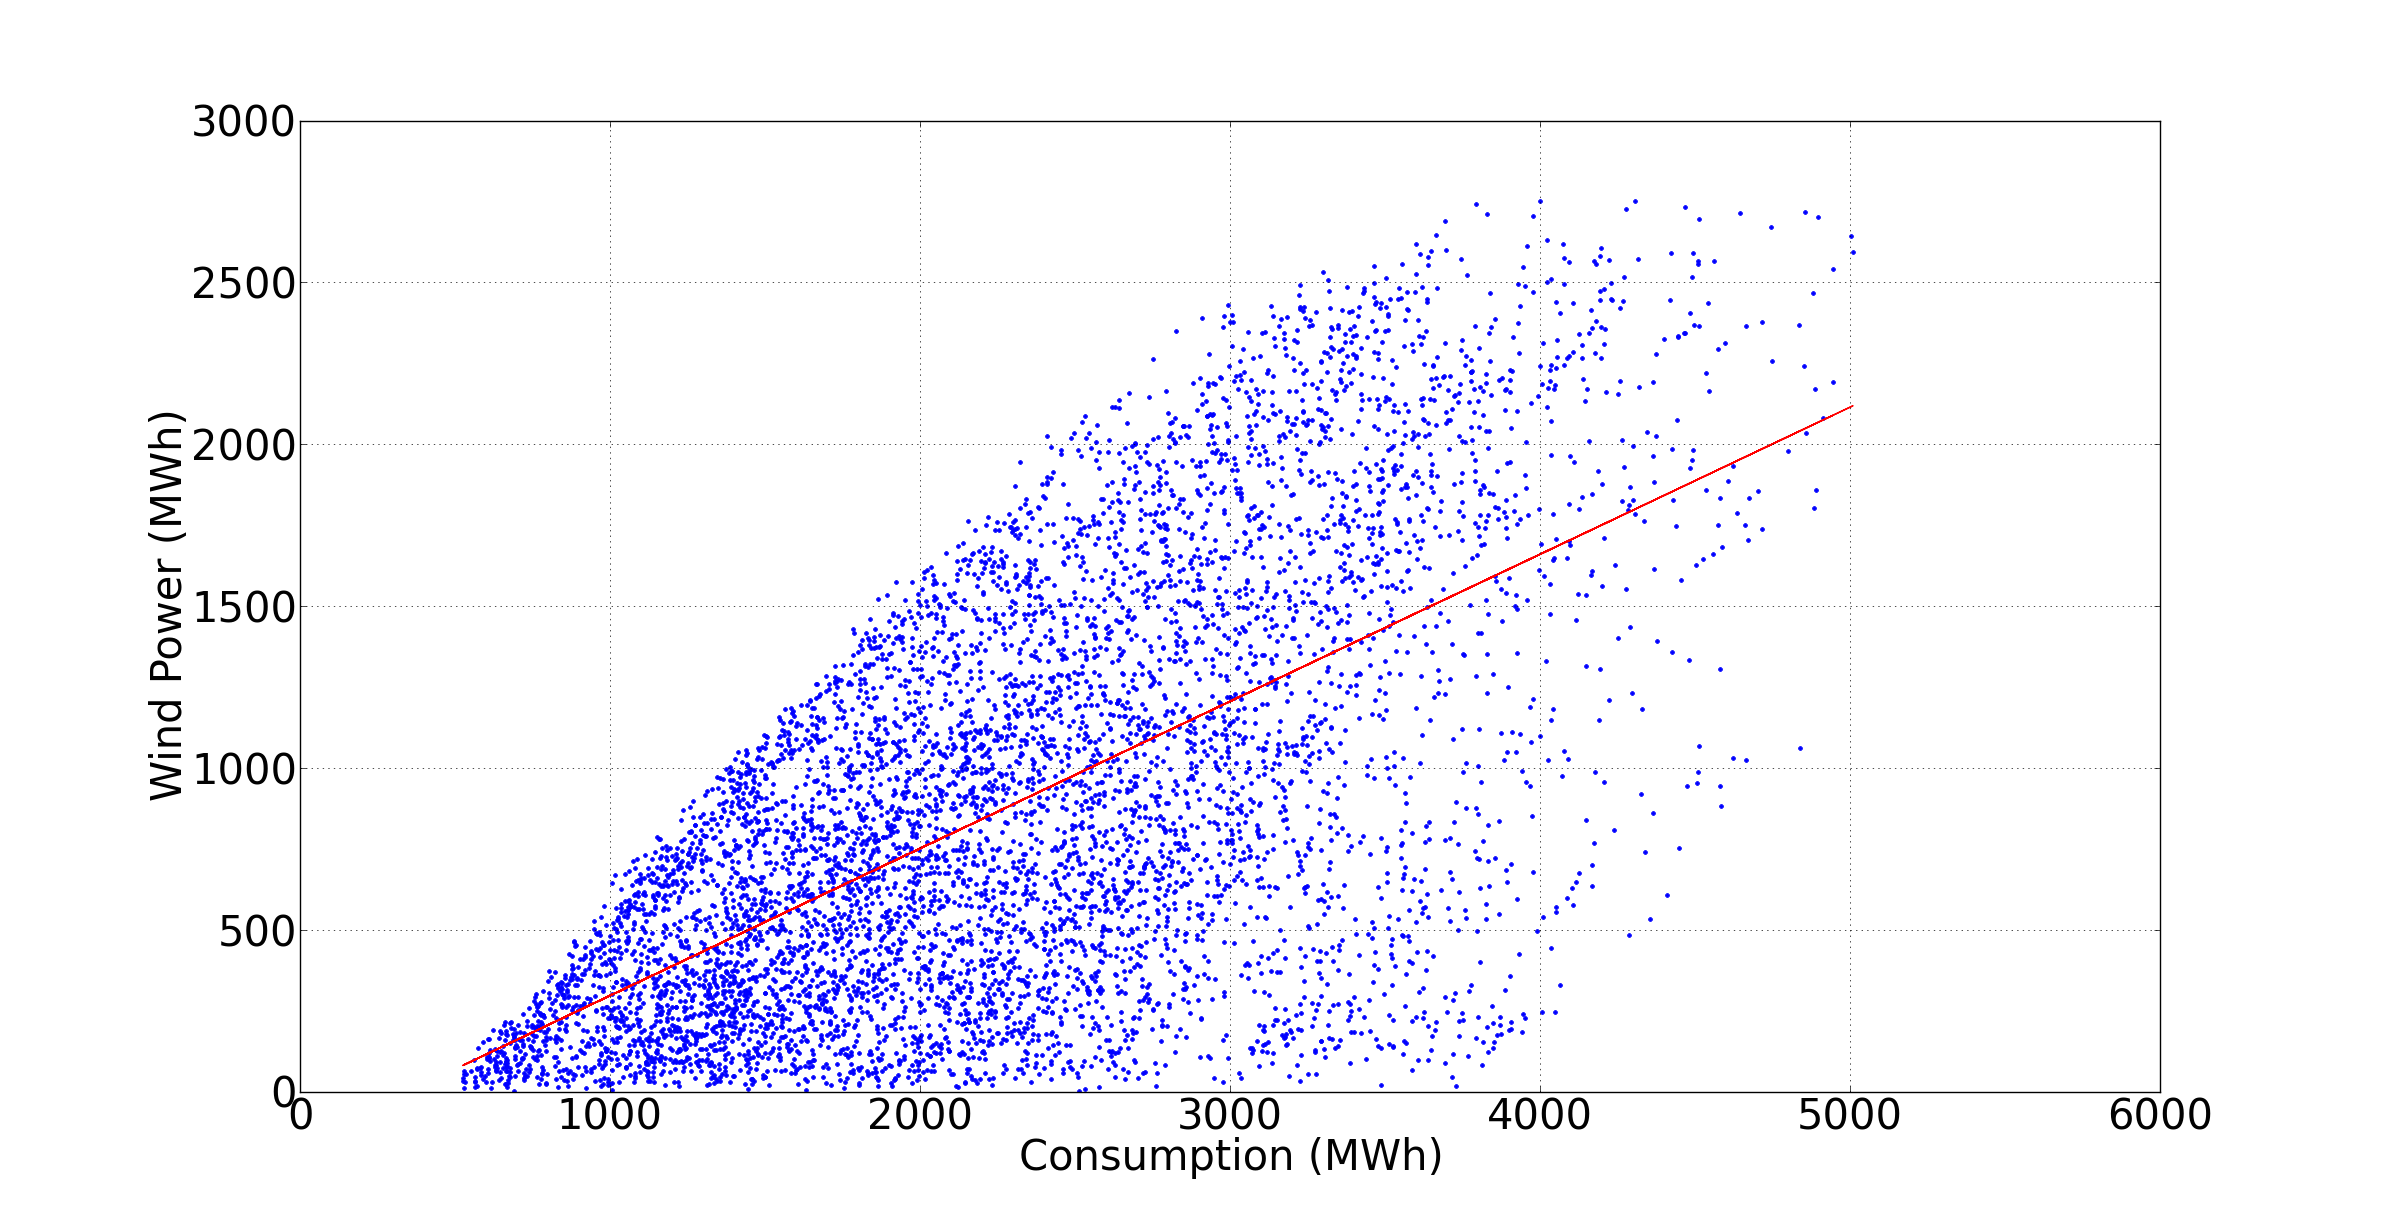
\includegraphics[width=0.95\linewidth]{billeder/consumptionVsWindProduction.png}
\caption{Demand vs. Wind Production in 2012}
\label{fig:demandVsWindProduction}
\end{figure}

\noindent Demand would be a predicted value in our ANN if used in a real setting. In our experiments we use actual values from nord pool spot to simulate the demand input --- it is out of scope for this thesis to predict it. A final remark is the potential of substituting demand with temperature because it is highly influenced by Heating Degree and Cooling Degree Days as presented in Section~\ref{sec:ElectricityDemand}. The relationship between temperature and demand is expressed in Figure~\ref{fig:consump_temp_green} and we will investigate if this substitution is possible. This must be mentioned in relation to the absence of predicted demand because using the actual value makes the substitution less likely --- in a real life setting the demand would be predicted based on temperature (and other meteorological factors) which could potentially be directly substituted in the network instead of the prediction. What speaks for temperature as a substitution is that it in one parameter can reflect both demand and air density and thereby make the network more simple. We will compare the two approaches in experiments to come. 

\begin{figure}[H]
\centering
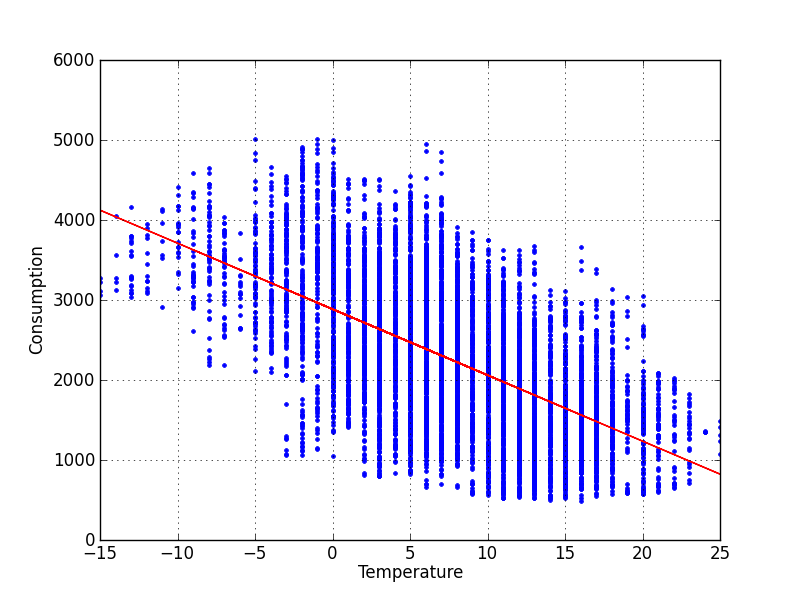
\includegraphics[width=0.95\linewidth]{billeder/energy_price_plots/consump_temp.png}
\caption{Demand and temperature plot.}
\label{fig:consump_temp_green}
\end{figure}

\subsubsection{Time of day}
\label{sec:greenTOD}
The dataset used for prediction consists of hourly observations for all calendar days of the year. It is worth identifying if there is a pattern within these days. The time of day an its associated average wind power is illustrated in the pillar diagram of Figure~\ref{fig:hourly_wind_production}. During 2012 the hours between 8-20 have a higher wind power production in general. It indicates what have been stated before with the correlation to demand, namely the amount of wind power is adjusted to the actual market demand. Time of day will be included in the experiments to verify the connection that has been established here. 

\begin{figure}[H]
\centering
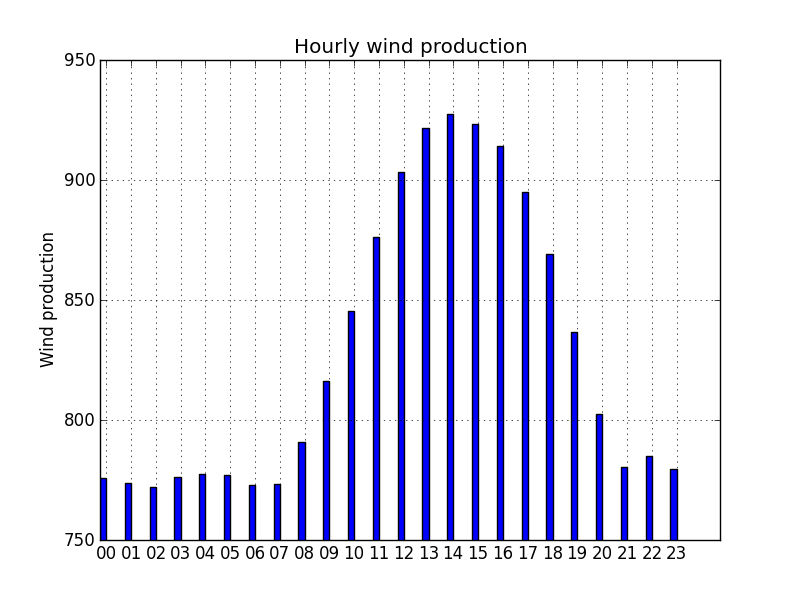
\includegraphics[width=0.8\linewidth]{billeder/hourly_wind_production.png}
\caption{Time of day vs. Wind Production in 2012}
\label{fig:hourly_wind_production}
\end{figure}

\subsection{Seasonality}
\label{sec:windProdSeasonality}
The wind speed follows seasonal changes. It is highly probable that the wind power on the market will follow this change due to its obvious relation to wind speed. Figure~\ref{fig:windProductionMonths} visualizes this relationship for the different months of 2012. The wind power is lower from April to August compared to all other months of the year. A clear distinction between the actual seasons can be seen in the pillar diagram of Figure~\ref{fig:windProductionSeasons} where the former is confirmed with summer and spring being lowest in wind power. Seasonality must be considered as input and tested in experiments.

\begin{figure}[H]
\centering
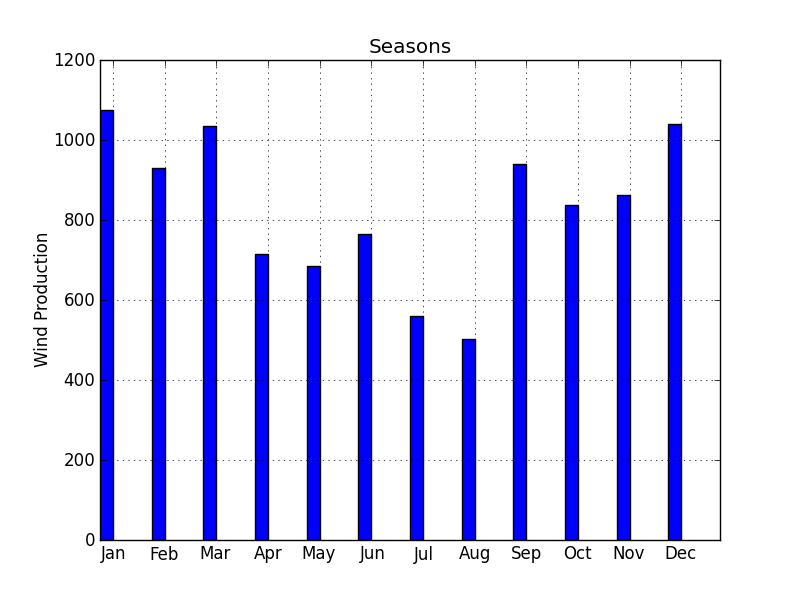
\includegraphics[width=0.85\linewidth]{billeder/Seasons/windProductionMonths.png}
\caption{Wind production in relation to months in 2012}
\label{fig:windProductionMonths}
\end{figure}

\begin{figure}[H]
\centering
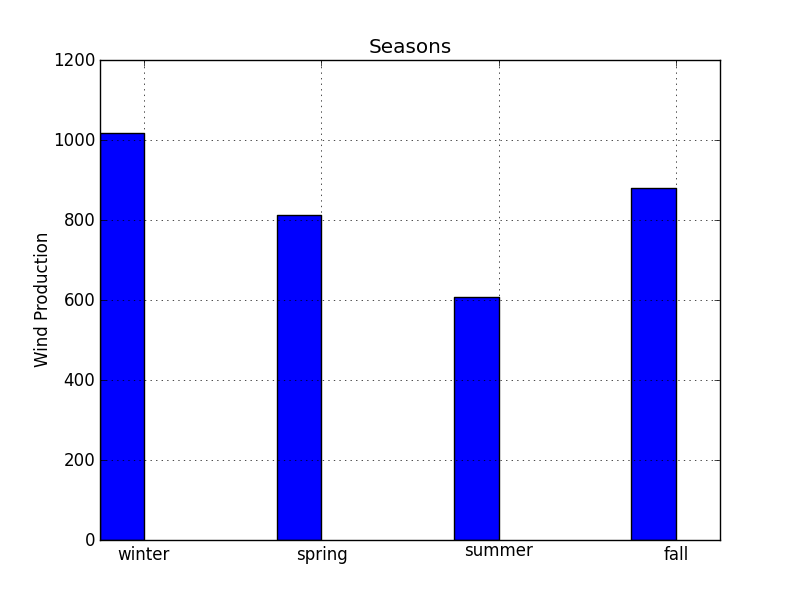
\includegraphics[width=0.85\linewidth]{billeder/Seasons/windProdctionSeasons.png}
\caption{Wind production in relation to the four seasons in 2012}
\label{fig:windProductionSeasons}
\end{figure}

\subsection{Wind Production Development}
\label{sec:windProductionDev}
The above analysis shows the wind production development to be much dependent on wind speed and air density together with the general trend on the market in relation to demand. 
\\[0.5cm]
Wind power is highly volatile. This statement is clear when observing the development curve for the first 400 of a year in Figure~\ref{fig:windHourDevelopment400Hours} --- these hours are much representative for the overall development of wind power. 

\begin{figure}[H]
\centering
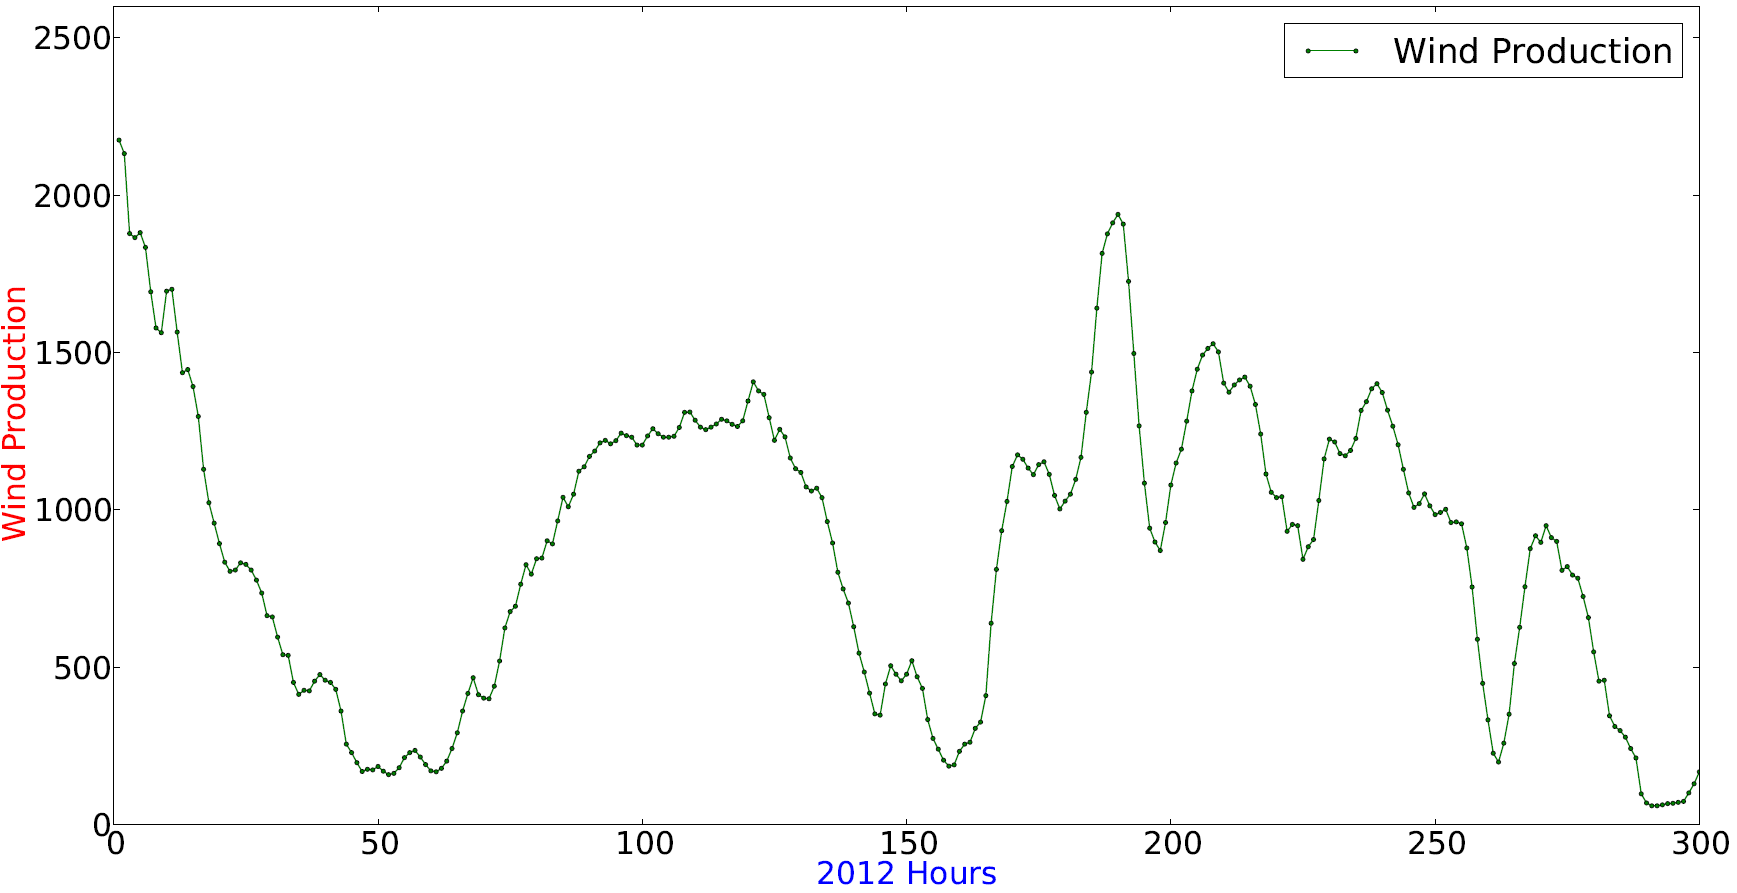
\includegraphics[width=0.99\linewidth]{billeder/productionTendency400Hours.png}
\caption{Wind production development for 400 hours in 2011}
\label{fig:windHourDevelopment400Hours}
\end{figure}

\noindent We hope to predict 24-hours ahead and in order to do so we must be able to identify the trends of the dataset, e.g. are we moving up or down based analysing the previous hours. The issue is discussed in detail in Section~\ref{sec:usingStatisticalInput} but in short more characteristics about trends in the dataset will allow us to approach our target more accurately. The ANN function can run into problem when trying to generalize on meteorological factors alone due to the many wind power productions associated with the same wind speed. Hopefully consumption and air density can help wind speed within this interval but attempting to add even more information of wind power is worth a try. To exemplify consider a situation where similar inputs (in this case temperature, demand and wind speed) will result in many different wind power productions during the year. The similar days are defined by having similar wind speeds, temperatures and demands during the day --- the margins for what defines a similar days can be seen in Table~\ref{table:similarHoursLimitsWindProd} just below.

\begin{table}[H]
\centering  % used for centering table
\begin{tabular}{|c|c|c|c|} % centered columns (3 columns)
\hline
 & \#1 Windspeed & \#2 Temperature (Celsius) & \#3 Demand \\ \hline % inserts table 
High margin: & 16.5 & 3.3 & 2359.5  \\ \hline
Low margin: & 13.5 & 2.7 & 1930.5 \\ \hline % [1ex] adds vertical space
\hline %inserts single line
\end{tabular}
\caption{This is the high and low margins used for the the similar input to output distribution.} % title of Table
\label{table:similarHoursLimitsWindProd} % is used to refer this table in the text
\end{table}

\noindent The similar days result in an amount of different wind power productions which also emphasizes its volatility. The different productions can be seen in Figure~\ref{fig:inputParameterDistribution} and range from 848-1398. The generalization will move towards 848-1048 within this interval but if we are facing a similar day during prediction but on a rising trend with a value of 1198 coming just before then we would still guess between 848-1048 instead of the higher value that is much more likely. The point of the simple example is to illustrate the importance of considering the the immediate previous hours because of their significant for the movements to come. Identifying these previous movements will give us the possibility of a more accurate prediction. The simplest way to include information about the past is to include the wind power from past hours and let the network itself calculate the impact of former wind power productions --- Figure~\ref{fig:windProductionVsLastWindProduction} shows the relationship between the current production and the last known production with a Pearson constant being 0,99   

\begin{figure}[H]
\centering
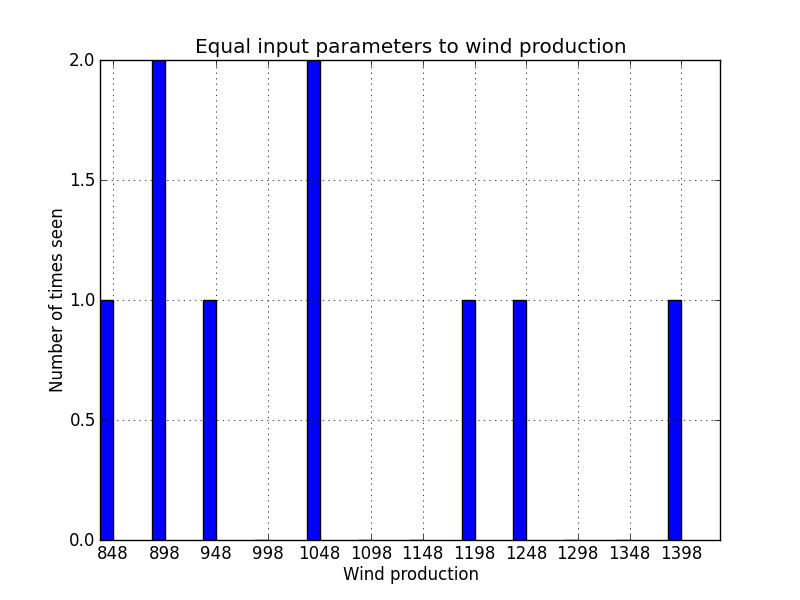
\includegraphics[width=0.85\linewidth]{billeder/Equal_wind.png}
\caption{Same input parameter to wind production output distribution}
\label{fig:inputParameterDistribution}
\end{figure}

\begin{figure}[H]
\centering
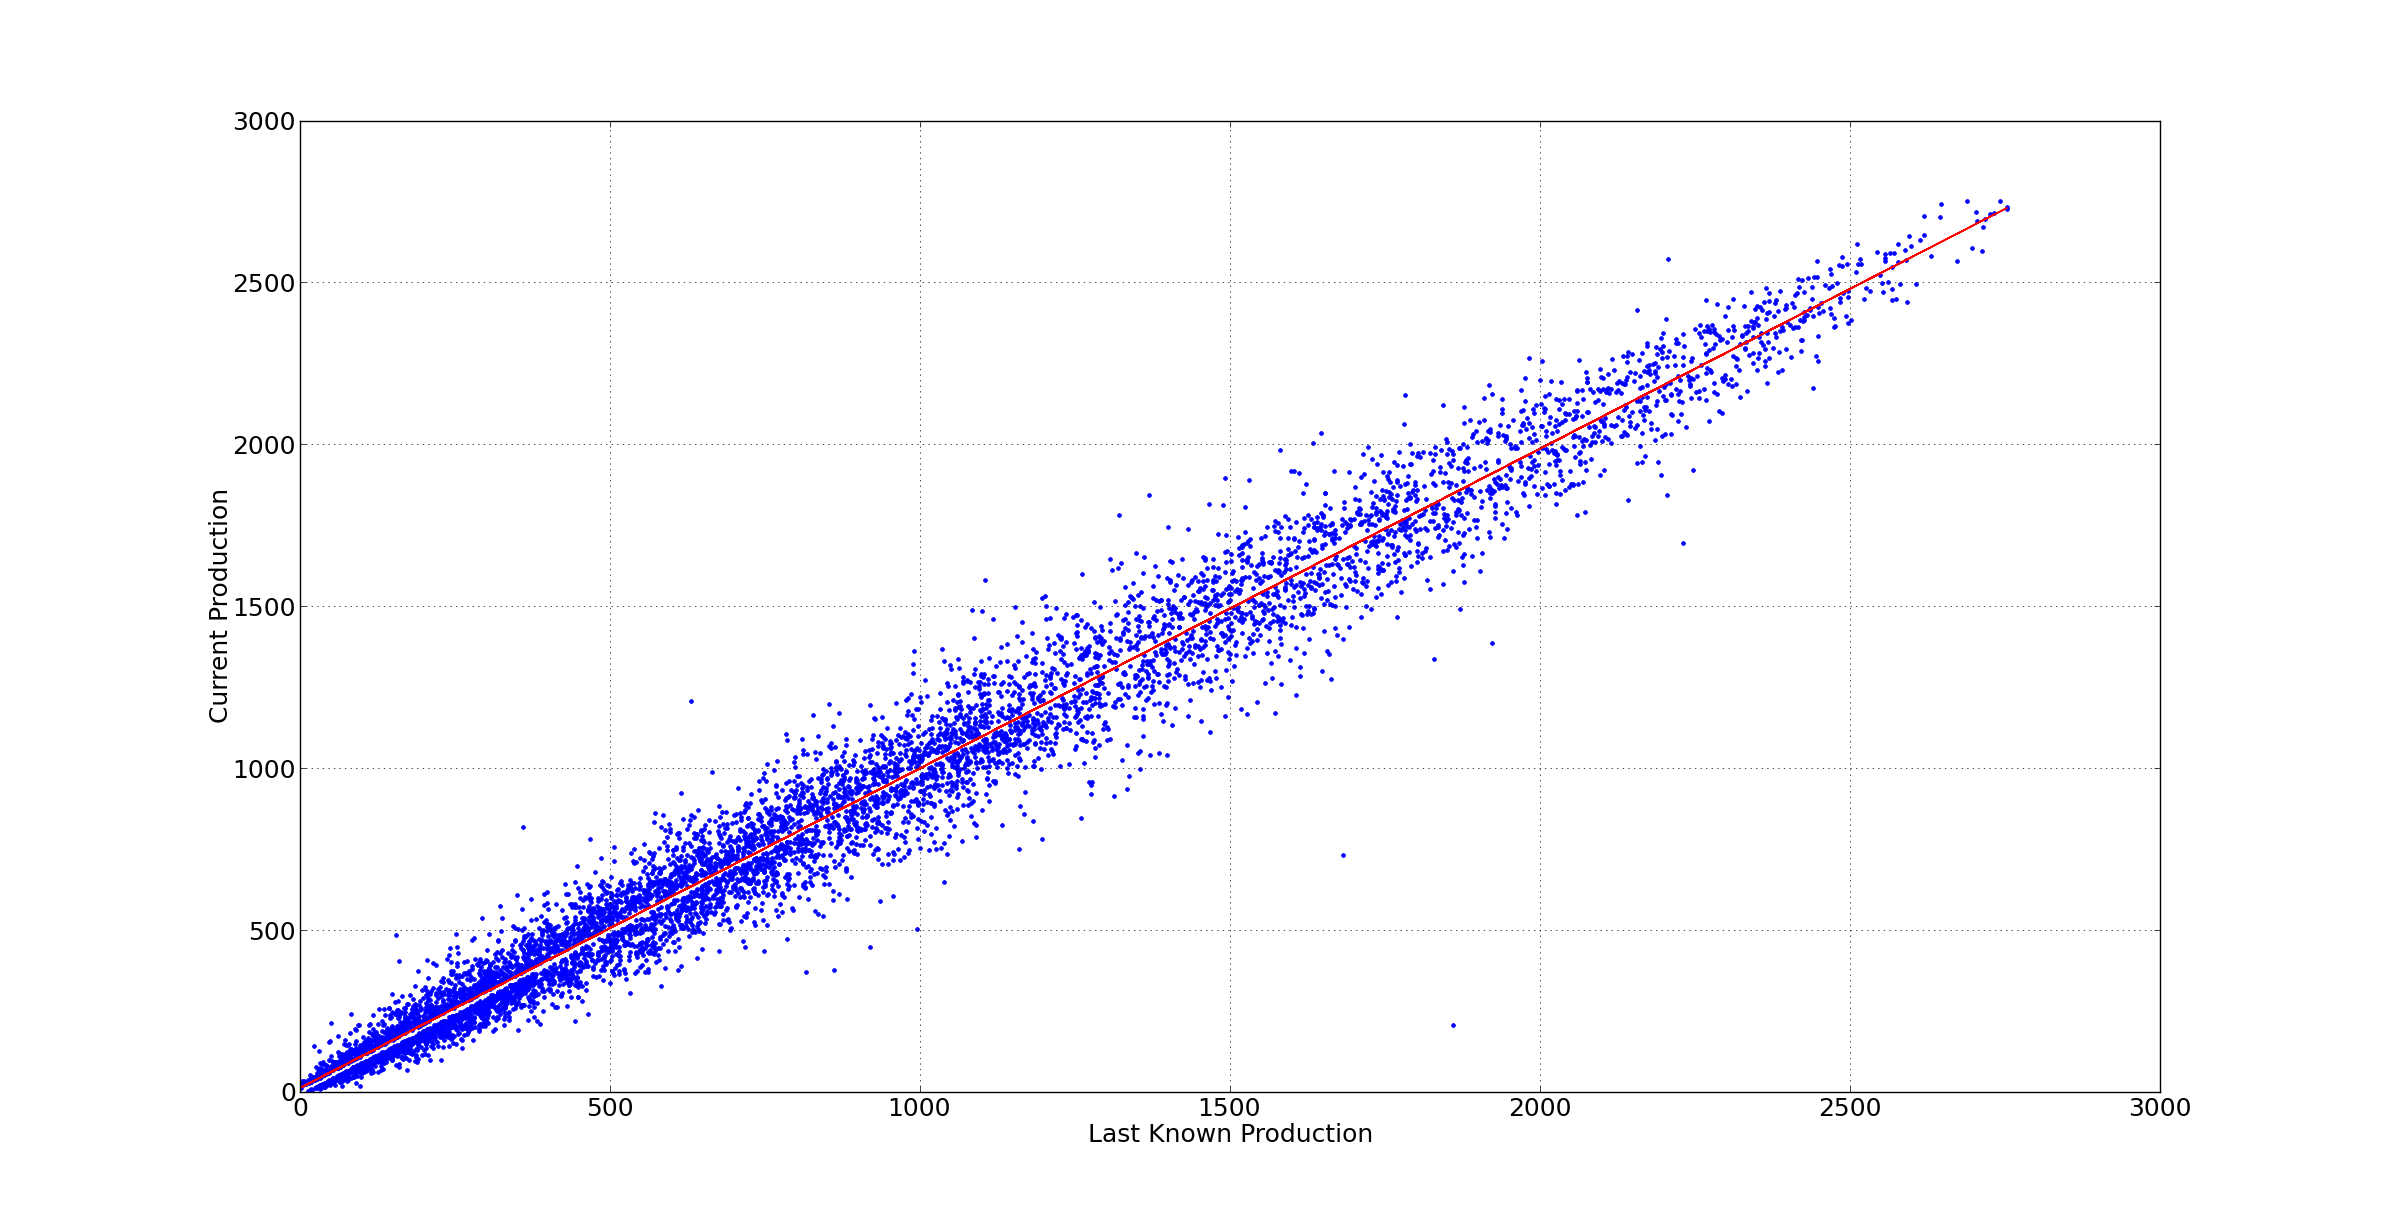
\includegraphics[width=0.95\linewidth]{billeder/windProductionVsLastWindProduction.png}
\caption{Wind power vs. last known wind power}
\label{fig:windProductionVsLastWindProduction}
\end{figure}

\noindent The relationship between the individual calculated approaches and wind power will not be analysed further here due to the many adjustable settings in the calculations (different hours and smoothing factor as described in Section~\ref{sec:usingStatisticalInput}) but the analysis show the potential for capturing trendlike behaviour throughout the dataset which will be tested in the experiments.

\subsubsection{Trimming} 
Trimming is for removing irregularities that we are not able to predict. Intuitively this makes no sense for wind power since it is constrained by natural forces and the windmills ability to produce power --- at some point nothing more can be produced. What could give rise to irregularities is the wind power and its connection to the electricity market where a sudden rise in demand could result in the need for pushing a huge amount of power into the market. Figure~\ref{fig:windProductionTrimming} attempts to illustrate the different hours that would be cut off when using percentile trim. The most noticeable thing is that a larger trim will cut the tops of the graphs which could potentially result in the creation of irregularities. 

\begin{figure}[H]
\centering
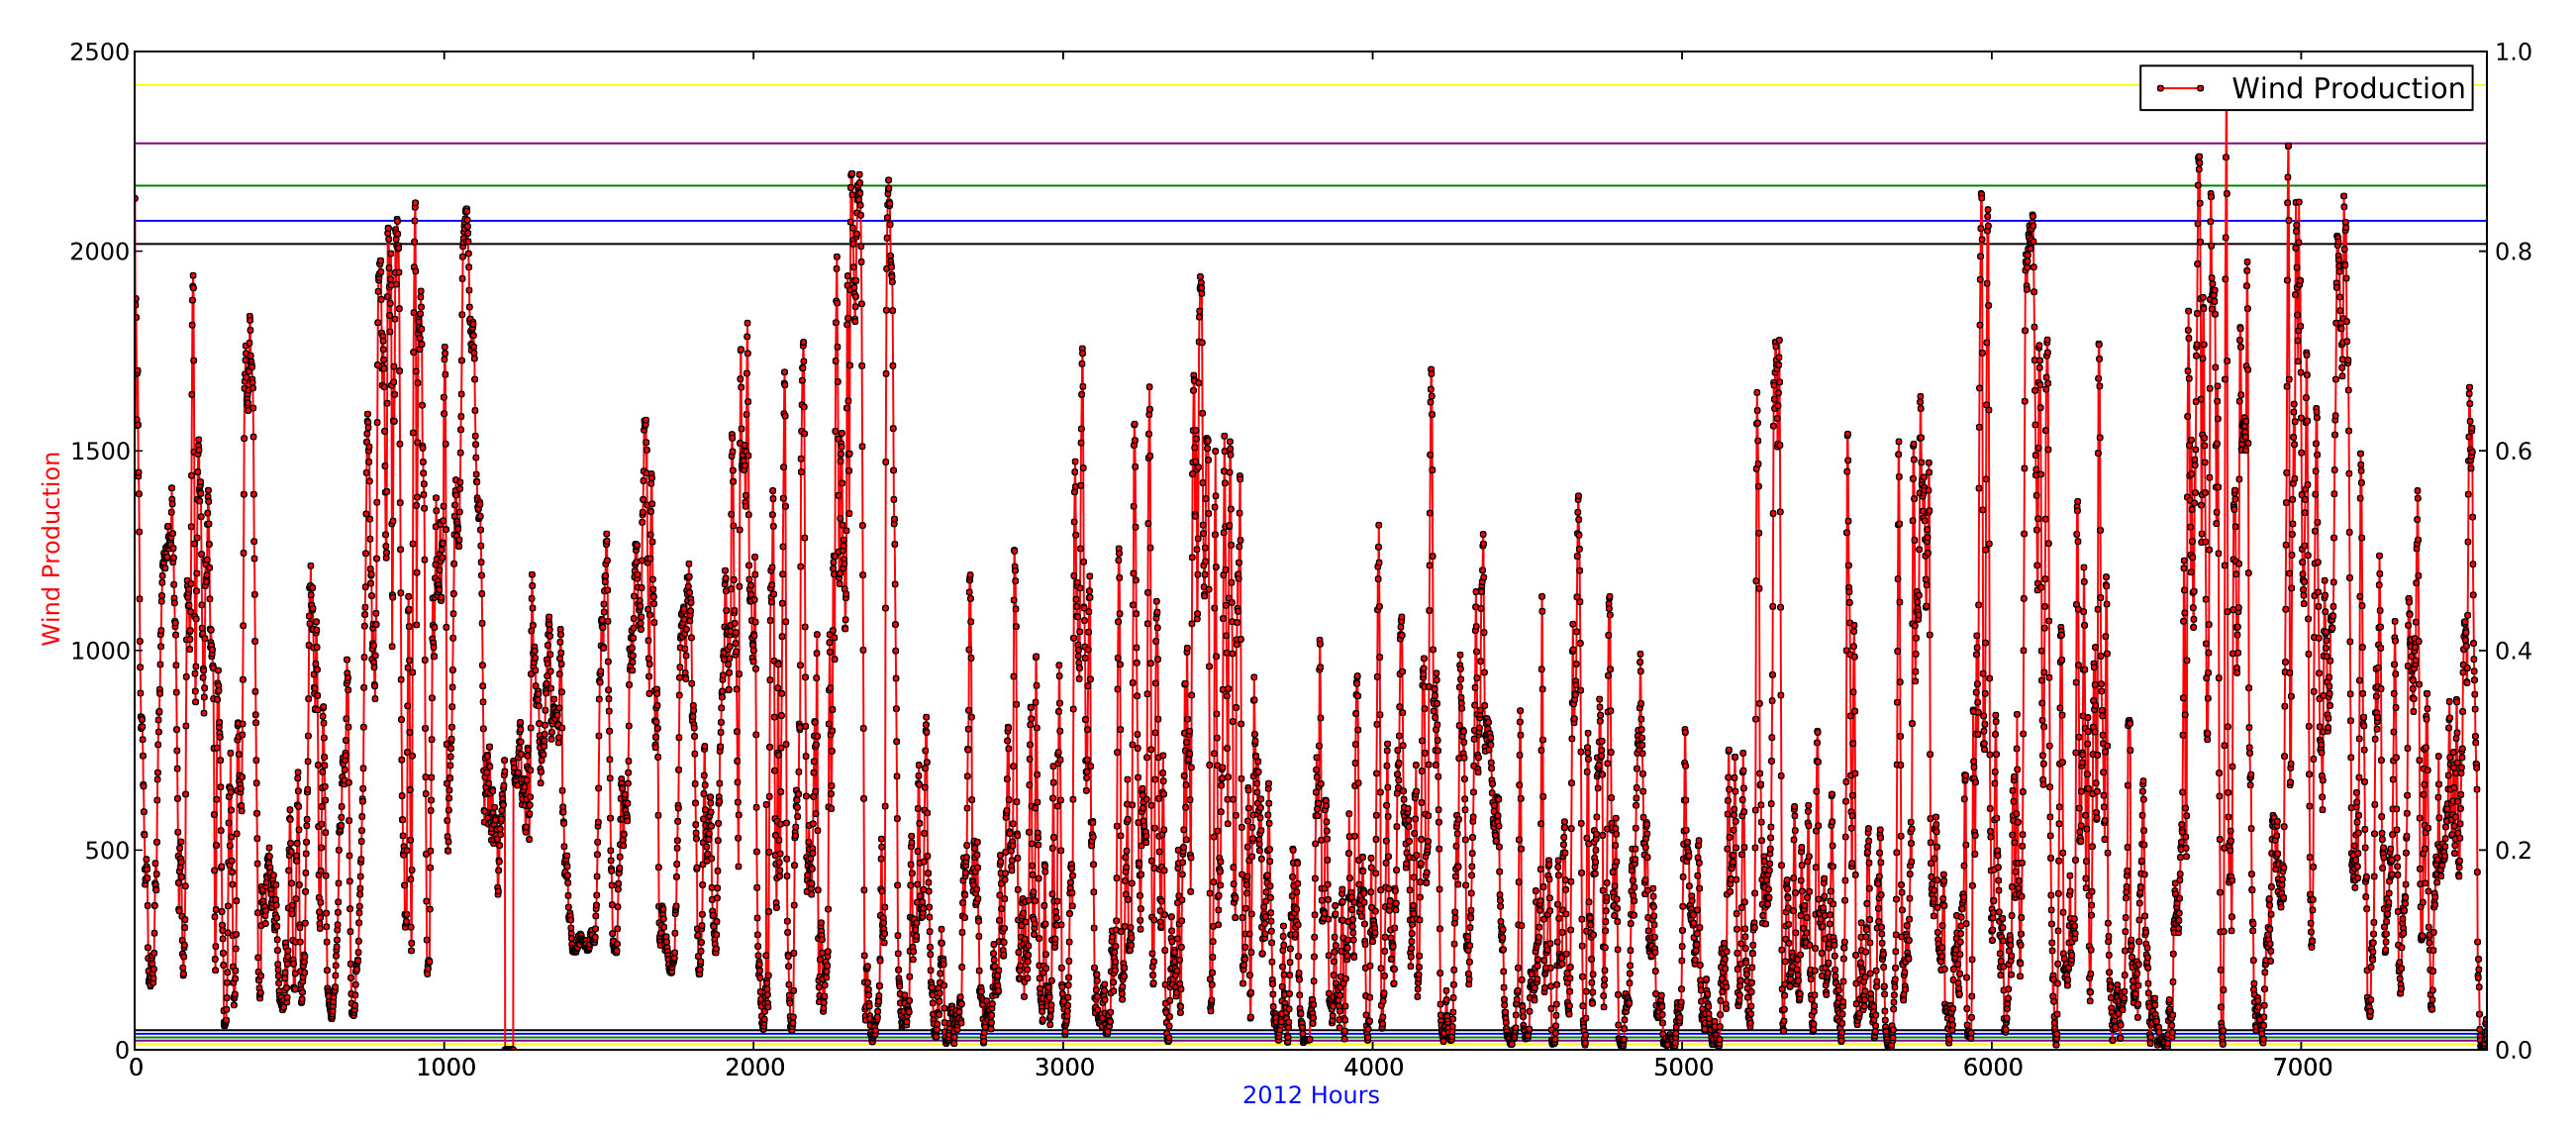
\includegraphics[width=0.99\linewidth]{billeder/windProductionTrimming.jpg}
\caption{Wind power production trimming}
\label{fig:windProductionTrimming}
\end{figure}

The graph containing the trims for the entire year makes it hard to see what is actually cut-off but is still gives the sense of potential values being removed from the dataset. The graph in Figure~\ref{fig:pointingOutPlaceWhereTrim} highlights the ours between 6200-7200 to give a better sense of what is removed. It is observable that there are not sudden drops but all wind power productions have intermediary steps --- we want to be able to predict all of these values and since they are not irregular it makes no sense to remove them. The only irregularity we can identify happens in around 1100 in Figure~\ref{fig:windProductionTrimming} where the wind power suddenly drops to zero, e.g. we will require the values to be above zero. It will be discussed later if it in the hands of a trader could make sense to trim data based on expertise, e.g. if the trader has knowledge about trend movements and experience tells that within the next 24 hours only certain values are plausible to occur then trimming could be a possibility. It will of course only make sense if trimming away values do not create more noise and achieves more accuracy but this will be tested in experiments.

\begin{figure}[H]
\centering
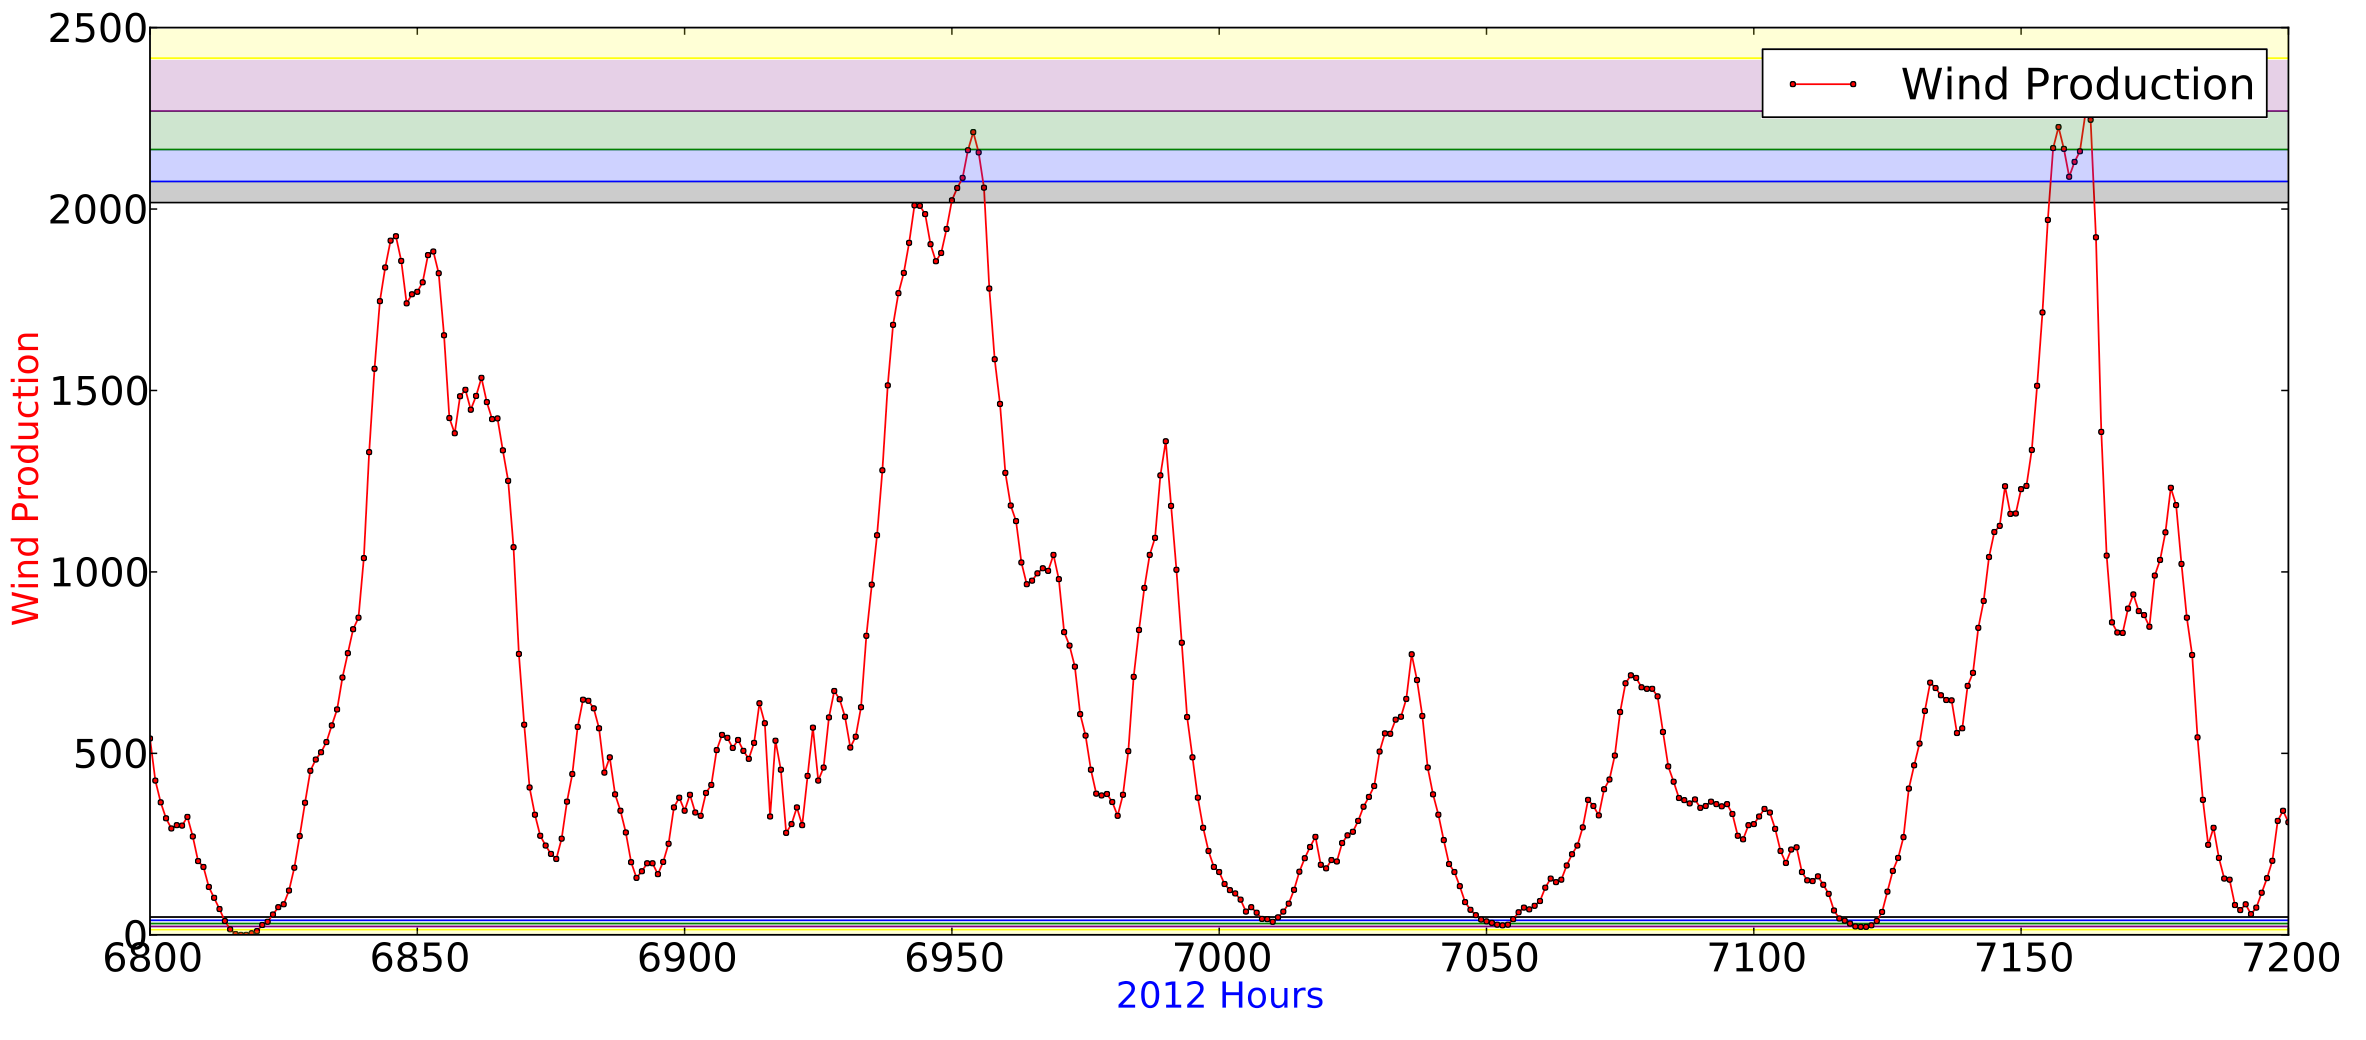
\includegraphics[width=0.99\linewidth]{billeder/pointingOutPlaceWhereTrim.png}
\caption{Wind power production vs. last known wind power production}
\label{fig:pointingOutPlaceWhereTrim}
\end{figure}

\subsection{Conclusion}
The above analysis has clarified to what extend the different parameters affect the wind power. Not surprisingly wind speed has the greatest influence on wind power, but also demand has shown a good correlation with the production which suggest a close link to the electricity market. The wind power vary from hour to hour (highest between 8-20) which makes the time of day a significant factor. The wind power is decreased significantly during winter so the season will also need to be included in test. The analysis of the yearly wind power development showed the need for including past wind power production to better identify the movements to come.
The air density is according to its formula proportional to wind power and it showed a correlation of 0,28 in average which makes it applicable for testing. The current wind direction and wind power is related with a correlation of 0,21 but further validation needs to be carried out in experiments.